
\documentclass[
	11pt
	   t,
	aspectratio=169
]{beamer}

\graphicspath{{img/}}

\usepackage[alf]{abntex2cite}
\usepackage{booktabs} 
\usepackage{palatino} 
\usepackage[default]{opensans}
\usepackage{subcaption}
\usepackage[utf8]{inputenc}
\usepackage[russian]{babel}
\usepackage{pgfplots}
\pgfplotsset{width=8cm,compat=1.9}
\usepgfplotslibrary{external}
\tikzexternalize
\usepackage[utf8]{inputenc}
\usepackage{listings}
\usepackage{xcolor}

\definecolor{vscBackground}{RGB}{255,255,255}    
\definecolor{vscKeyword}{RGB}{175,0,219}         
\definecolor{vscString}{RGB}{163,21,21}          
\definecolor{vscComment}{RGB}{0,128,0}           
\definecolor{vscFunction}{RGB}{121,94,38}        
\definecolor{vscNumber}{RGB}{9,134,88}           
\definecolor{vscOperator}{RGB}{175,0,219}        
\definecolor{vscText}{RGB}{0,0,0}                
\definecolor{vscLineNr}{RGB}{128,128,128}        

\lstset{
    inputencoding=utf8,
    extendedchars=true,
    literate=%
        {á}{{\'a}}1 {é}{{\'e}}1 {í}{{\'i}}1 {ó}{{\'o}}1 {ú}{{\'u}}1
        {Á}{{\'A}}1 {É}{{\'E}}1 {Í}{{\'I}}1 {Ó}{{\'O}}1 {Ú}{{\'U}}1
        {à}{{\`a}}1 {è}{{\`e}}1 {ì}{{\`i}}1 {ò}{{\`o}}1 {ù}{{\`u}}1
        {À}{{\`A}}1 {È}{{\'E}}1 {Ì}{{\`I}}1 {Ò}{{\`O}}1 {Ù}{{\`U}}1
        {ã}{{\~a}}1 {ẽ}{{\~e}}1 {ĩ}{{\~i}}1 {õ}{{\~o}}1 {ũ}{{\~u}}1
        {Ã}{{\~A}}1 {Ẽ}{{\~E}}1 {Ĩ}{{\~I}}1 {Õ}{{\~O}}1 {Ũ}{{\~U}}1
        {â}{{\^a}}1 {ê}{{\^e}}1 {î}{{\^i}}1 {ô}{{\^o}}1 {û}{{\^u}}1
        {Â}{{\^A}}1 {Ê}{{\^E}}1 {Î}{{\^I}}1 {Ô}{{\^O}}1 {Û}{{\^U}}1
        {ç}{{\c c}}1 {Ç}{{\c C}}1
        {º}{{\textordmasculine}}1
        {ª}{{\textordfeminine}}1
}

\lstdefinestyle{baseStyle}{
    backgroundcolor=\color{vscBackground},
    basicstyle=\ttfamily\small\color{vscText},
    breakatwhitespace=false,
    breaklines=true,
    captionpos=b,
    keepspaces=true,
    numbers=left,
    numbersep=5pt,
    showspaces=false,
    showstringspaces=false,
    showtabs=false,
    tabsize=4,
    frame=single,
    framerule=0.8pt,
    rulecolor=\color{gray!20},
    numberstyle=\tiny\color{vscLineNr},
    basicstyle=\footnotesize\ttfamily,
    keywordstyle=\bfseries\color{green!40!black},
    commentstyle=\itshape\color{purple!40!black},
    identifierstyle=\color{blue},
    stringstyle=\color{orange},
    columns=flexible,
    basewidth={0.5em,0.45em},
    inputencoding=utf8,
    extendedchars=true
}

%----------------------------------------------------------------------------------------
% C++
%----------------------------------------------------------------------------------------
\lstdefinestyle{cppStyle}{
    style=baseStyle,
    language=C++,
    morekeywords={class,private,protected,public,template,typename,namespace,
                  using,new,delete,this,friend,virtual,override,final,explicit,
                  mutable,constexpr,nullptr,noexcept,static_cast,dynamic_cast,
                  const_cast},
    morekeywords=[2]{cout,cin,endl,vector,string,map,set,queue,stack,pair,
                     begin,end,push_back,pop_back,emplace_back,size,empty},
    keywordstyle=[2]\color{vscFunction},
    sensitive=true
}

\lstnewenvironment{cpp}[1][]{\lstset{style=cppStyle, #1}}{}
\newcommand{\cppinline}[1]{\lstinline[style=cppStyle]!#1!}
\newcommand{\inputcpp}[2][]{\lstinputlisting[style=cppStyle,#1]{#2}}


\usetheme{Boadilla} 

\definecolor{primaryColor}{RGB}{20,45,105}
\definecolor{secondaryColor}{RGB}{0,100,160} 

\setbeamercolor{structure}{fg=primaryColor}
\setbeamercolor{palette primary}{bg=primaryColor, fg=white}
\setbeamercolor{palette secondary}{bg=secondaryColor, fg=white}
\setbeamercolor{title}{bg=primaryColor, fg=white}

\setbeamercolor{headline}{bg=secondaryColor, fg=white}
\setbeamercolor{section in head/foot}{bg=primaryColor, fg=white}
\setbeamercolor{subsection in head/foot}{bg=secondaryColor, fg=white}

\setbeamercolor{author in head/foot}{bg=primaryColor, fg=white}
\setbeamercolor{title in head/foot}{bg=secondaryColor, fg=white}
\setbeamercolor{date in head/foot}{bg=primaryColor, fg=white} 
\setbeamercolor{page number in head/foot}{bg=primaryColor, fg=white}

\useinnertheme{circles}
\useoutertheme{miniframes}
\setbeamertemplate{navigation symbols}{}


\title[Титул кратко]{Титул Полностью}
\author[Плотников Д.М., Закарлюка И.В. ]{Плотников Даниил Михайлович, Закарлюка Иван Владимирович} 
\institute[СПбГУ]{Санкт-Петербургский Государственный Университет} 
\date[Год]{} 

%------------------

\begin{document}

\begin{frame}
	\titlepage
\end{frame}

\begin{frame}
	\frametitle{Оглавление}
	\tableofcontents 
\end{frame}

\section{Пример}

%------------------------------------------------

\begin{frame}
	\frametitle{Обычный текст}
    Обычный текст пишется так

    \textbf{Вот так}

    \Huge 

    И даже так

    \tiny может и вот так

    \normalsize
    И в конце концов снова так
\end{frame}

%------------------------------------------------

\begin{frame}
	\frametitle{Списки}
    \begin{enumerate}
        \item Один
        \item Два
    \end{enumerate}

    \begin{itemize}
        \item Один
        \item Два
    \end{itemize}
\end{frame}

%------------------------------------------------

\begin{frame}[fragile]
	\frametitle{Код}
    не забудь [fragile]
    коменты не работают
\begin{cpp}
cout << "Python is bad\n";
\end{cpp}
	
\end{frame}

%------------------------------------------------

\begin{frame}
	\frametitle{Картинки}
    \center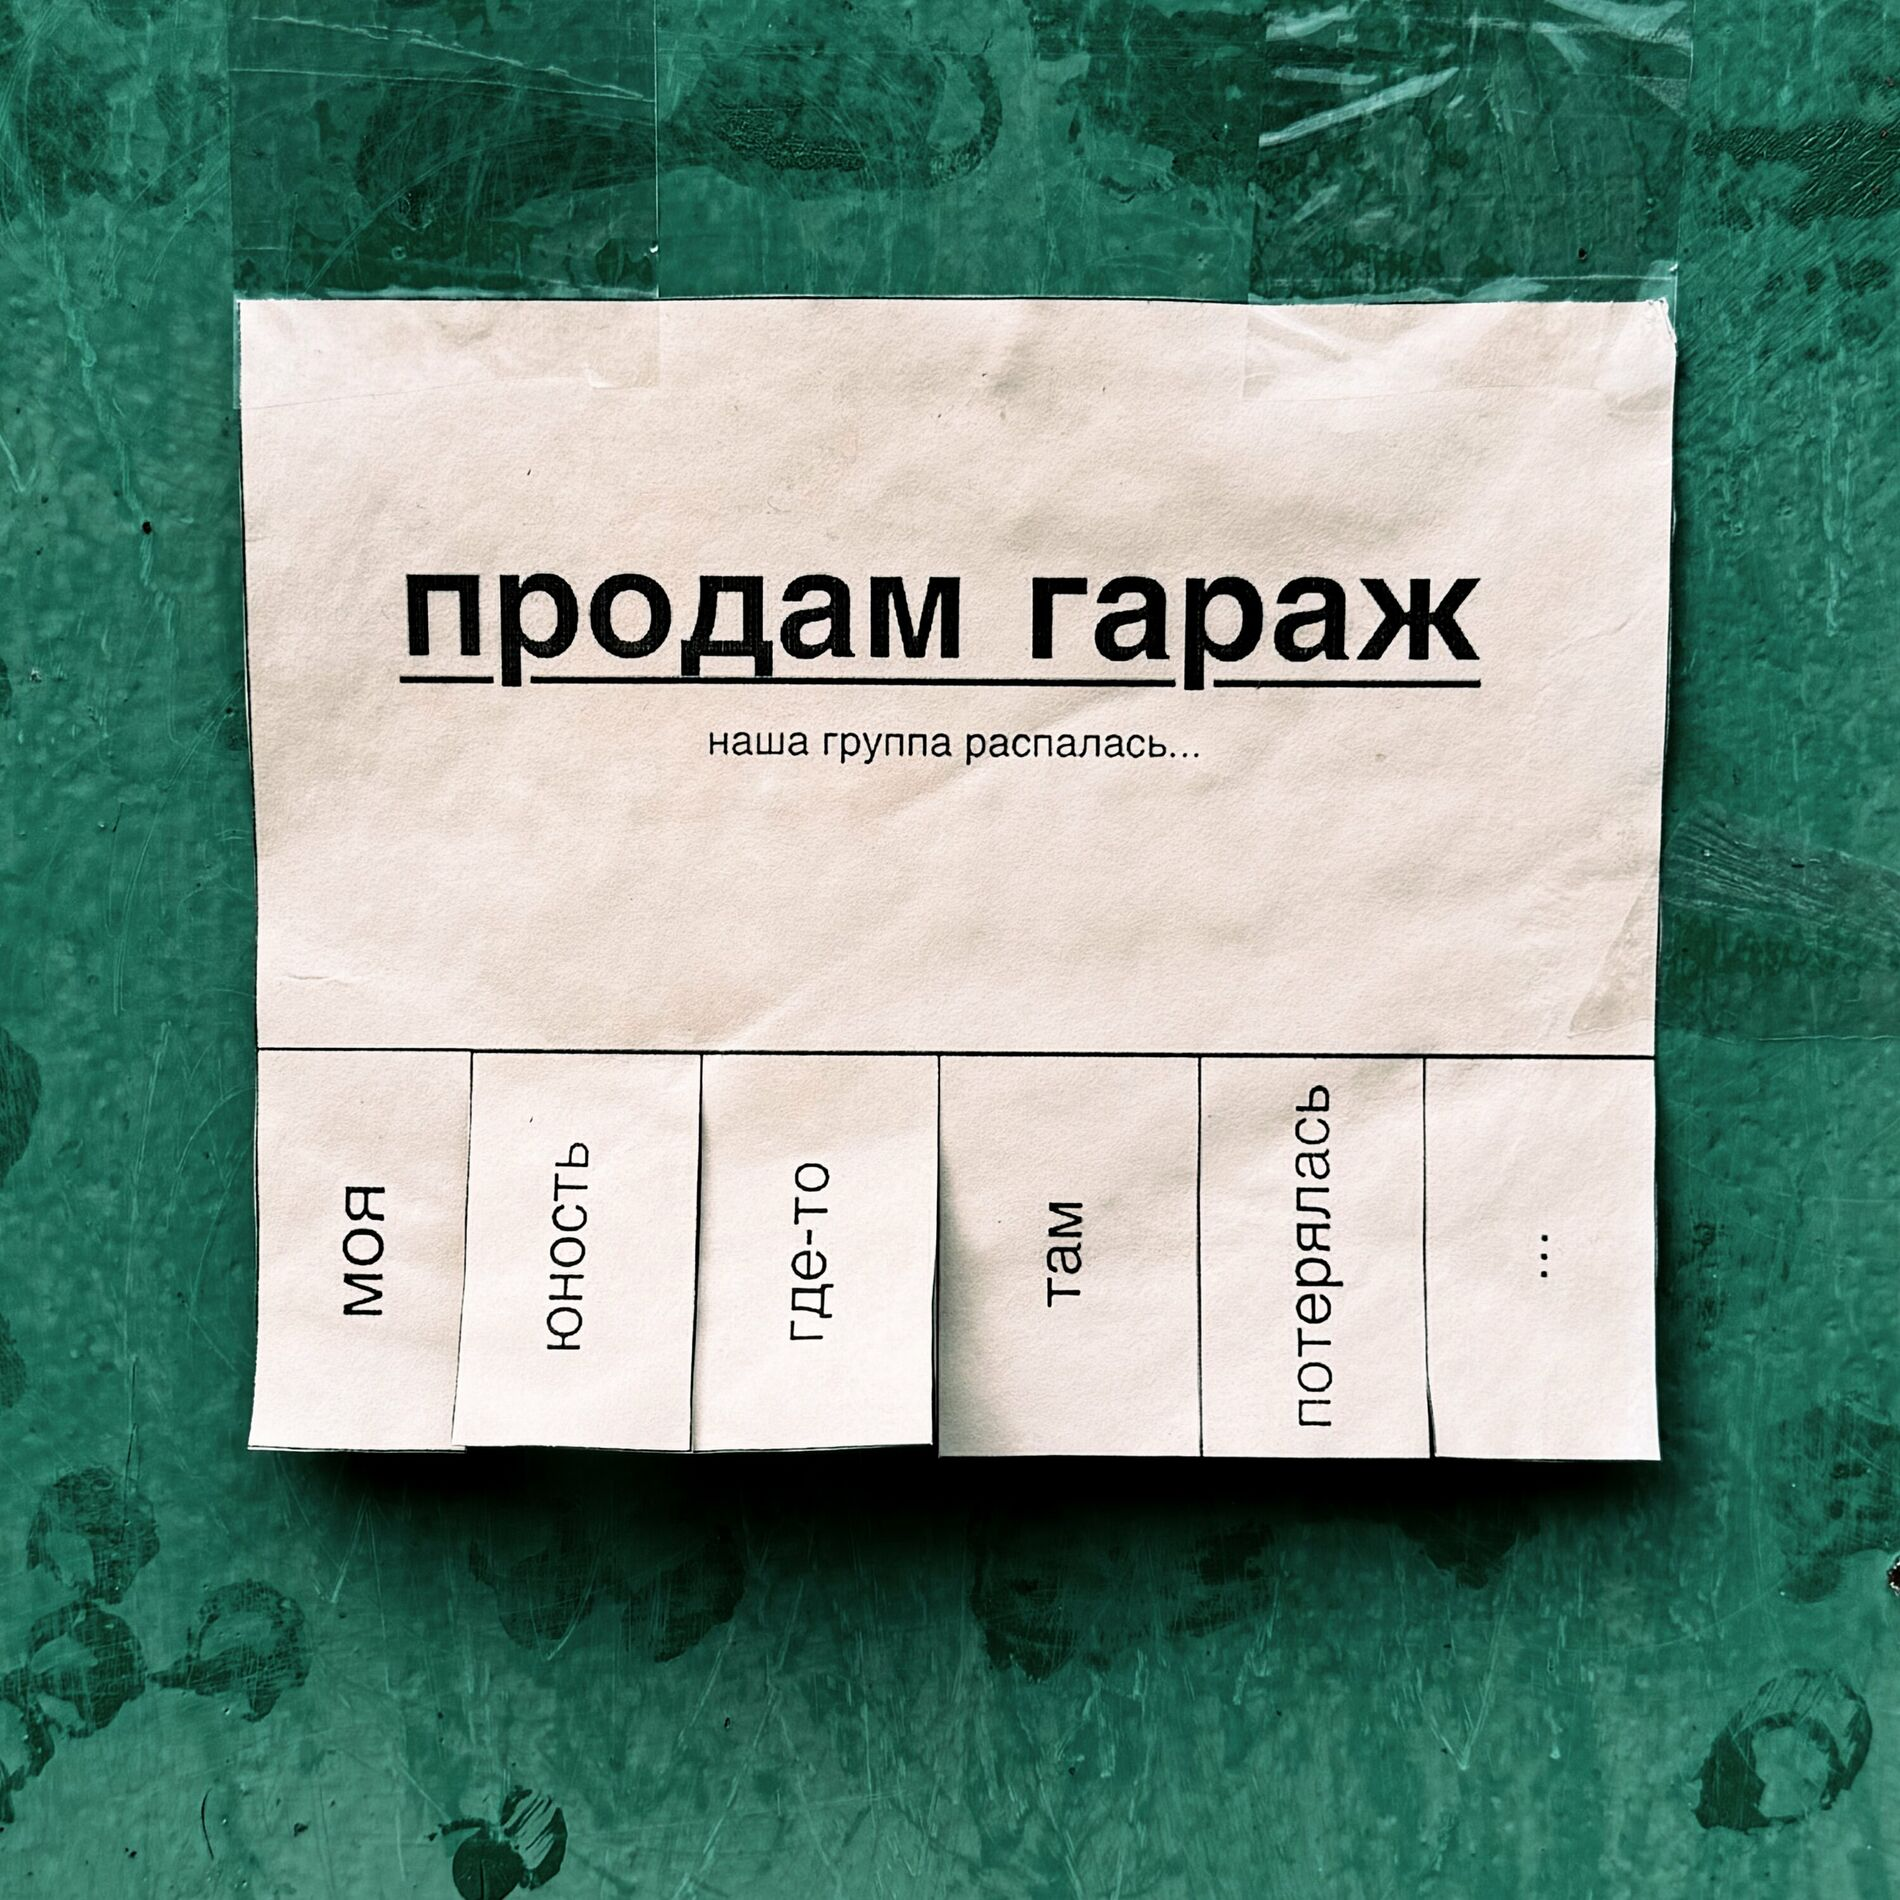
\includegraphics[scale=0.4]{image.jpg}

\end{frame}

%------------------------------------------------

\begin{frame}
	\frametitle{Графики}
	
    \begin{tikzpicture}
        \begin{axis}[
            xmin=0, xmax=100,
            ymin=0, ymax=20,
            xtick={0,100},
            ytick={0,120},
            legend pos=north east,
            ]

            \addplot[
                color=blue,
                mark=none,
                samples=200,
                domain=0:100,
                unbounded coords=jump
                ]
                {sqrt(x)};

            \addplot[
                color=red,
                mark=none,
                samples=200,
                domain=0:100,
                unbounded coords=jump
                ]
                {x};

            \legend{$\sqrt(x)$, 
                    $x$}
        \end{axis}
    \end{tikzpicture}
\end{frame}


%------------------

\end{document}

